\documentclass[final, 9pt, svgnames]{beamerPerdy}
\usetheme[
    titleformat title=smallcaps,
    progressbar=frametitle,
    numbering=fraction
]{metropolis}

\usetikzlibrary{positioning,fit,arrows.meta}

%\setbeameroption{show notes on second screen=right}

\setdefaultlanguage{english}

% Comando para usar comentarios
\newcommand{\comment}[1]{\textcolor{comment}{\footnotesize{#1}\normalsize}}

\newcommand\ImageNode[3][]{
    \node[draw=mLightBrown,line width=1pt,#1] (#2) {\includegraphics[width=1cm,height=1cm]{#3}};
}


\title{Packaging and Distributing}
\subtitle{Create, package and distribute your own python application}
\author[J. A. Perdiguero López]{
José Antonio Perdiguero López\\
\href{http://www.perdy.top}{\scriptsize{\faGlobe\; http://www.perdy.top}}\\
\href{https://github.com/PeRDy}{\scriptsize{\faGithub\; https://github.com/PeRDy}}\\
\href{https://www.linkedin.com/in/perdy}{\scriptsize{\faLinkedin\; https://www.linkedin.com/in/perdy}}\\
\scriptsize{\faAt\; perdy.hh@gmail.com}}
\date{September 24, 2017}
\institute[Piksel]{Lead Developer @ Piksel, Machine Learning Team}

\begin{document}

% Title
\begin{frame}[noframenumbering, plain]
    \titlepage
\end{frame}

% Index
\begin{frame}[noframenumbering, plain]{Index}
    \begin{columns}[t]
        \begin{column}{5cm}
            \setbeamertemplate{section in toc}[circle]
            \tableofcontents[sections={1-2}]
        \end{column}
        \begin{column}{5cm}
            \setbeamertemplate{section in toc}[circle]
            \tableofcontents[sections={3-5}]
        \end{column}
    \end{columns}
\end{frame}

% Introduction 
\section{Introduction}
\subsection{Why should I distribute my application?}
\begin{frame}{Why should I distribute my application?}
    \begin{itemize}
        \item Given enough eyeballs, all bugs are shallow.
        \item Upstream improvements.
        \item Force multiplier.
        \item Modular.
        \item Great advertising.
        \item Attract talent.
        \item Stand on the shoulders of giants.
        \item Best technical interview possible.
        \item Show your code.
    \end{itemize}
    \note{
        Si uno usa software open source, es del interés de todos contribuir. De esta forma, la cantidad de desarrolladores de cada proyecto es enorme, incrementando la cantidad de ideas para nuevas funcionalidades, ojos para detectar bugs, la riqueza y calidad del código... Dada la naturaleza de las contribuciones a estos proyectos, suelen estar bien modularizados.

    Los desarrolladores que contribuyen en proyectos open source suelen responder al perfil de desarrolladores con ganas de enfrentarse a problemas por solucionar. Esto, sumado a que puedes evaluar a un desarrollador por el código con el que ya ha contribuído a tus proyectos, es un aliciente para las empresas.
    }
    \footnotetext[1]{\href{https://opensource.com/life/15/12/why-open-source}{https://opensource.com/life/15/12/why-open-source}}
\end{frame}

\subsection{Versioning}
\begin{frame}{Versioning}
    \begin{block}{Version schema}
        A normal version must be denoted by \texttt{X.Y.Z} where \texttt{X}, \texttt{Y} and \texttt{Z} are positive integers. \texttt{X} represents the major version, \texttt{Y} the minor version and \texttt{Z} the patch version. Version \texttt{1.0.0} defines the public API.
    \end{block}

    \begin{block}{Version upgrade}
        Given a version number, increment:
        \begin{description}
            \item[Major] version when you make incompatible API changes. Reset minor and patch version to \texttt{0}.
            \item[Minor] version when you add functionality in a backwards-compatible manner. Reset patch version to \texttt{0}.
            \item[Patch] version when you make backwards-compatible bug fixes.
        \end{description}
    \end{block}
    \footnotetext[1]{\href{http://semver.org/}{http://semver.org/}}
    \note {
        Breve resumen del SemVer. 
        \begin{description} 
            \item[Major] cambios incompatibles en la API pública. 
            \item[Minor] nuevas funcionalidades. 
            \item[Patch] bugfixing.
        \end{description}
    }
\end{frame}

\subsection{Tools}
\begin{frame}{Tools I}
    \begin{block}{Prospector}
        Static code analysis using different tools.
        \href{https://github.com/landscapeio/prospector}{https://github.com/landscapeio/prospector}
    \end{block}
    \pause
    \begin{block}{Sphinx}
        Create documentation for your project.
        \href{https://github.com/sphinx-doc/sphinx}{https://github.com/sphinx-doc/sphinx}
    \end{block}
    \pause
    \begin{block}{Bumpversion}
        Utility to upgrade your project version.
        \href{https://github.com/peritus/bumpversion}{https://github.com/peritus/bumpversion}
    \end{block}
    \pause
    \begin{block}{Pre-commit}
        Utility that does some checks before git commits.
        \href{https://github.com/pre-commit/pre-commit}{https://github.com/pre-commit/pre-commit}
    \end{block}
\end{frame}
\begin{frame}[fragile]{Tools II}
    \begin{block}{Tox}
        Run your tests using many different python interpreters.
        \href{https://github.com/tox-dev/tox}{https://github.com/tox-dev/tox}
    \end{block}
    \pause
    \begin{block}{Cookiecutter}
        Application that creates project skeletons using Jinja templates.
        \href{https://github.com/audreyr/cookiecutter}{https://github.com/audreyr/cookiecutter}
    \end{block}
    \pause
    \begin{block}{Cookiecutter Template}
        Cookiecutter template for Python packages.
        \href{https://github.com/PeRDy/cookiecutter-python-package}{https://github.com/PeRDy/cookiecutter-python-package}
    \end{block}
    \pause
    \begin{block}{Clinner}
        Utility to create powerful Command Line Interfaces with a few lines.
        \href{https://github.com/PeRDy/clinner}{https://github.com/PeRDy/clinner}
    \end{block}
    \note{
        \begin{description}
            \item[Tox] facilita la ejecución de tests bajo diferentes intérpretes de Python.

            \item[Cookiecutter] se encarga de crear fácilmente la estructura de un proyecto desde cero.

            \item[Clinner] es la piedra angular del proceso de crear un paquete, testearlo y distribuirlo. La plantilla genera una aplicación de línea de comando que permite simplificar el proceso de construcción. La documentación se puede consultar en ReadTheDocs.
        \end{description}
    }
\end{frame}

\begin{frame}{Services}
    \begin{block}{PyPI}
        Python Package Index, the main repository of python software.
        \href{https://pypi.python.org/pypi}{https://pypi.python.org/pypi}
    \end{block}
    \pause
    \begin{block}{GitHub}
        Repositories for your source code.
        \href{https://github.com}{https://github.com}
    \end{block}
    \pause
    \begin{block}{Travis}
        Continuous Integration service.
        \href{https://travis-ci.org/}{https://travis-ci.org/}
    \end{block}
    \pause
    \begin{block}{Codecov}
        Keeps the changes of test coverage of your code.
        \href{https://codecov.io}{https://codecov.io}
    \end{block}
    \pause
    \begin{block}{ReadTheDocs}
        Stores and serves documentation for your project.
        \href{https://readthedocs.io}{https://readthedocs.io}
    \end{block}
    \note{
        Alternativas a GitHub: \emph{Bitbucket}, \emph{Gitlab}.

        \emph{Travis} y \emph{Codecov} son gratis para proyectos open source.
    }
\end{frame}

% Creation
\section{Creation}
\subsection{Storing the project}
\begin{frame}{Storing the project}
    \begin{figure}
        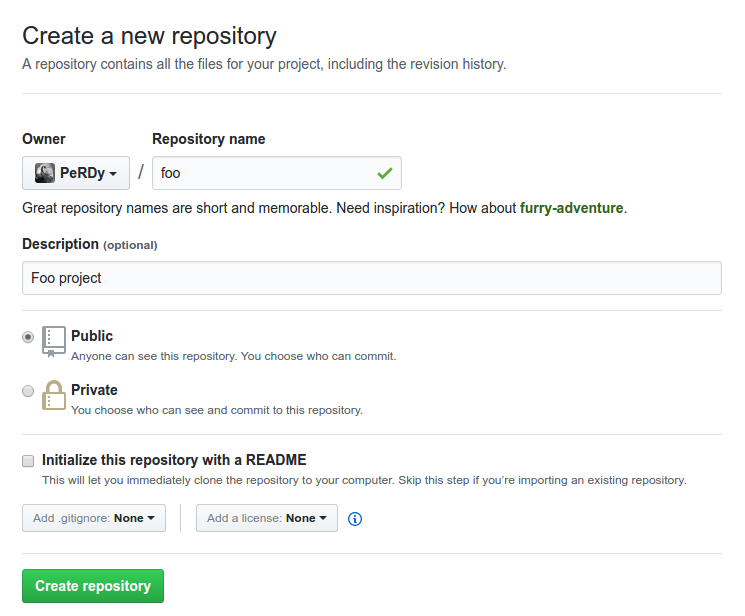
\includegraphics[width=\textwidth,height=0.8\textheight,keepaspectratio]{create_repository.png}
    \end{figure}
    \note{
        Esta charla está completamente orientada a open source así que, ¿por qué no trabajar con GitHub?
    }
\end{frame}

\subsection{Create the project skeleton}
\begin{frame}[fragile]{Create the project skeleton}
    \begin{block}{Cookiecutter context}
        Define all variables needed by cookiecutter to properly create the project skeleton, these variables can be found in \textit{cookiecutter.json} file.
    \end{block}
    \pause
    \begin{block}{Create skeleton}
        Execute cookiecutter with previously defined context to create the project skeleton.
    \end{block}
    \pause
    \begin{block}{Commit \& push}
        Time to do your first commit and push to repository:
        \begin{minted}{bash}
git remote add origin git@github.com:PeRDy/foo.git
git commit -a -m "Initial commit"
git push
        \end{minted}
    \end{block}
    \note {
        Para crear el proyecto:
        \begin{enumerate}
            \item Definir el contexto necesario para Cookiecutter: nombre, autor, repositorio...
            \item Crear el esqueleto del proyecto con la plantilla.
            \item Commit iniciar y pushear.
        \end{enumerate}
    }
\end{frame}

\subsection{Project hierarchy}
\begin{frame}{Project hierarchy}
    \begin{columns}
        \begin{column}{0.2\textwidth}
            \begin{figure}
                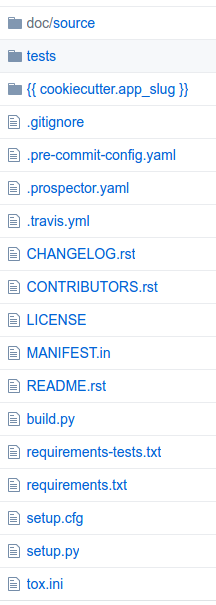
\includegraphics[width=\textwidth,height=\textheight,keepaspectratio]{project_skeleton.png}
            \end{figure}
        \end{column}
        \begin{column}{0.80\textwidth}
            \begin{block}{Documentation folder}
                The place that keeps all the documentation source files as well as the doc config file.
            \end{block}
            \pause
            \begin{block}{Tests folder}
                All tests files are stored in a tests folder where tests collectors can gather them without problems.
            \end{block}
            \pause
            \begin{block}{Application folder}
                The application itself, the \emph{python package} distributed, and the same that other users will import in their applications.
            \end{block}
            \pause
            \begin{block}{Root files}
                Files that keeps in the root directory are usually:
                \begin{itemize}
                    \item Tools configuration.
                    \item Services configuration.
                    \item Build scripts.
                    \item Metadata.
                \end{itemize}
            \end{block}
        \end{column}
    \end{columns}
    \note{
        \begin{description}
            \item[Configuración de herramientas] Prospector, Pre-commit, Git.
            \item[Configuración de servicios] Travis.
            \item[Scripts de construcción] \texttt{build.py}, \texttt{setup.py}, \texttt{tox.ini}.
            \item[Metadatos] Readme, manifest, contributors, changelog, requirements, \texttt{setup.cfg}.
        \end{description}
    }
\end{frame}

\begin{frame}[fragile]{Relevant files I}
    \begin{block}{Manifest}
        This file, \texttt{MANIFEST.in}, with own syntax\footnote[1]{\href{https://docs.python.org/3/distutils/commandref.html#sdist-cmd}{https://docs.python.org/3/distutils/commandref.html#sdist-cmd}} defines the directories and files that will be included in the distributable package.
    \end{block}
    \pause
    \begin{block}{Requirements}
        List all requirements of your project, that are added as dependencies when installed. Usually requirements are splitted in two files: \texttt{requirements.txt} for real dependencies and \texttt{requirements-tests.txt} for dependencies necessaries to test the project.
    \end{block}
    \pause
    \begin{block}{Metadata}
        Metadata files: \texttt{README.rst}, \texttt{CONTRIBUTORS.rst}, \texttt{CHANGELOG.rst} and \texttt{LICENSE}.
    \end{block}
    \note{
        El fichero README puede ser escrito en reStructuredText o en Markdown. Este fichero, renderizado, será la página principal del proyecto en GitHub,
    }
\end{frame}

\begin{frame}{Relevant files II}
    \begin{block}{Tools and Services config}
        Configuration files for tools and services: \texttt{setup.cfg}, \texttt{.pre-commit-config.yaml}, \texttt{.prospector.yaml}, \texttt{.travis.yml}, \texttt{.gitignore}.
    \end{block}
    \pause
    \begin{block}{Setup}
        Main file that defines how the project will be packaged, gather metadata from other files and provides an interface to create distributable packages.
    \end{block}
    \pause
    \begin{block}{Tox}
        Tox file, \texttt{tox.ini}, defines the environments and commands that tox executes. In this case, defines an environment for each python version that should be tested, another for run lint tools and the last one for compile documentation.
    \end{block}
    \note{
        El fichero principal de configuración es \texttt{setup.cfg}, que es un fichero de estilo \texttt{.ini}, dividido en secciones con configuraciones para las diferentes herramientas como por ejemplo \emph{bumpversion}, \emph{pytest} y \emph{coverage}.

        El fichero \texttt{setup.py} contiene la versión actual del proyecto, su nombre y su lista de requirements.

        Tox está integrado con Travis.
    }
\end{frame}
\begin{frame}{Relevant files III}
    \begin{block}{Build}
        The build file, \texttt{build.py}, is the entrypoint for everything related to build, including \emph{testing}, \emph{packaging} and \emph{distributing}. This is a command line application using \emph{Clinner} that provides a set of utility commands such as:
        \begin{itemize}
            \item Run tests and code coverage.
            \item Run lint.
            \item Run tox.
            \item Create documentation.
            \item Upgrade version, create package and upload to pypi.
        \end{itemize}
    \end{block}
    \note {
        Estas son las funciones del script de Clinner, más adelante se muestra la salida de la ayuda del script.
    }
\end{frame}

% Packaging
\section{Packaging}
\subsection{Test your application}
\begin{frame}[fragile]{Test your application}
    \begin{block}{Development}
        Run tests while developing using pytest.
        \begin{minted}{bash}
python build.py pytest
        \end{minted}
    \end{block}
    \pause
    \begin{block}{Multi-environment}
        Once development is done, run tests against all different interpreters supported to check compatibility.
        \begin{minted}{bash}
python build.py tox
        \end{minted}
    \end{block}
    \pause
    \begin{block}{Continuous Integration}
        Development is done, tests pass in every environment, so code can be uploaded to repository safely. Once a commit is done:
        \begin{description}
            \item[Travis] run tests in every environment and will notify in case any test didn't pass. When all tests pass,
            \item[Codecov] records current code coverage. In the same commit,
            \item[ReadTheDocs] gets the code, build docs and updates the project's doc page.
        \end{description}
    \end{block}
    \note {
        Testeamos en tres fases diferentes, con objetivos diferentes:
        \begin{enumerate}
            \item Development para comprobar que el código es correcto conforme a los tests.
            \item Multi-environment para comprobar que el código es correcto en diferentes intérpretes de python.
            \item CI para comprobar que la calidad del código y los tests no disminuye con nuevas versiones.
        \end{enumerate}
    }
\end{frame}

\subsection{Creating a package}
\begin{frame}[fragile]{Package types}
    \begin{block}{Egg}
        Source distribution.
        \begin{minted}{bash}
python setup.py sdist
        \end{minted}
    \end{block}
    \pause
    \begin{block}{Wheel}
        Built and binary distribution.
        \begin{minted}{bash}
python setup.py bdist_wheel
        \end{minted}
    \end{block}
    \note{
        Hay dos tipos de paquetes en Python: \emph{egg} y \emph{wheel}. 
        
        Los primeros, \emph{source distribution}, necesitan construirse al instalarlos. Los segundos, \emph{built or binary distribution}, simplemente necesitan ser movidos al directorio correcto. 
        
        Para entender la diferencia entre unos y otros, en cuanto a tiempo de instalación, podemos tomar como ejemplo \emph{numpy}, \emph{scipy} and \emph{pandas}.
    }
\end{frame}

\begin{frame}{Builder}
    \begin{figure}
        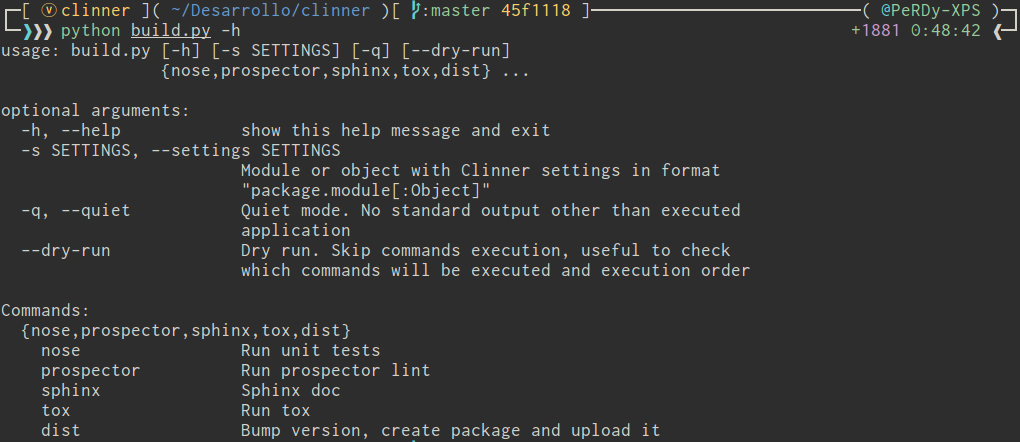
\includegraphics[width=\textwidth,height=0.8\textheight,keepaspectratio]{build_help.png}
    \end{figure}
    \note {
        Aquí se pueden ver las utilidades dentro del script \texttt{build.py}, entre las que encontramos comandos para:
        \begin{itemize}
            \item Generar la documentación.
            \item Realizar el análisis estático de código. 
            \item Lanzar los tests con pytest o con tox. 
            \item Empaquetar y distribuir la applicación.
        \end{itemize}
    }
\end{frame}


% Distributing
\section{Distributing}
\subsection{Register the application}
\begin{frame}[fragile]{Register the application}
    \begin{block}{PyPI account}
        Create a PyPI\footnote[1]{\href{https://pypi.python.org/pypi}{https://pypi.python.org/pypi}} account.
        Configure \texttt{.pypirc} file with PyPI credentials.
    \end{block}
    \pause
    \begin{block}{Application register}
        Use twine\footnote[2]{\href{https://github.com/pypa/twine}{https://github.com/pypa/twine}} with a package of your application to register it in PyPI:
        \begin{minted}{bash}
twine register dist/project-name.whl
        \end{minted}
    \end{block}
\end{frame}

\subsection{Upload a new version}
\begin{frame}[fragile]{Upload a new version}
    \begin{block}{Upload packages}
        Use twine again to upload all packages to PyPI:
        \begin{minted}{bash}
twine upload dist/project-name.whl
twine upload dist/project-name.tar.gz
        \end{minted}
    \end{block}
\end{frame}
 

% Conclusion
\section{Conclusion}
\subsection{Full workflow}
\begin{frame}[fragile]{Full workflow}
    \makebox[\textwidth][c]{
    \begin{tikzpicture}[
            node distance=0.8cm,
            >={Triangle[angle=60:1pt 2]},
            shorten >= 2pt,
            shorten <= 2pt,
            arrow/.style={
                ->,
                mLightBrown,
                line width=3pt
            }
        ]
        \ImageNode[label={Create Project}]{A}{python_logo.png}
        \ImageNode[label={Configure},right=of A]{B}{python_logo.png}
        \ImageNode[label={0:Code},right=of B]{C}{python_logo.png}
        \ImageNode[label={Upgrade Version},above right=of C]{D}{python_logo.png}
        \ImageNode[label={Package},right=of D]{E}{python_logo.png}
        \ImageNode[label={PyPI},right=of E]{F}{python_logo.png}

        \ImageNode[label={-90:GitHub},below right=of C]{G}{github_logo.png}
        \ImageNode[label={-90:Travis},right=of G]{H}{travis_logo.png}
        \ImageNode[label={-90:Codecov},right=of H]{I}{codecov_logo.png}
        \ImageNode[label={0:ReadTheDocs},below=of H]{J}{readthedocs_logo.png}

        \draw[arrow] (A) -- (B);
        \draw[arrow] (B) -- (C);
        \draw[arrow] (C) -- (D);
        \draw[arrow] (D) -- (E);
        \draw[arrow] (E) -- (F);
        \draw[arrow] (C) -- (G);
        \draw[arrow] (G) -- (H);
        \draw[arrow] (H) -- (I);
        \draw[arrow] (G) -- (J);

        \onslide<2->{
            \node (X) [draw=mLightGreen, fit= (A) (B), inner sep=0.55cm, thick, fill=mLightGreen, fill opacity=0.1] {};
            \node [yshift=1.5ex, mLightGreen] at (X.south) {Creation};
        }
        \onslide<3->{
            \node (Y) [draw=mLightGreen, fit= (D) (E) (F), inner sep=0.55cm, thick, fill=mLightGreen, fill opacity=0.1] {};
            \node [yshift=1.5ex, mLightGreen] at (Y.south) {Packaging \& Distributing};
        }
        \onslide<4->{
            \node (Z) [draw=mLightGreen, fit= (G) (H) (I) (J), inner sep=0.55cm, thick, fill=mLightGreen, fill opacity=0.1] {};
            \node [yshift=1.5ex, mLightGreen] at (Z.south) {Continuous Integration};
        }
    \end{tikzpicture}
    }
    \note {
        El desarrollo de una nueva funcionalidad se podría dividir en tres módulos:
        \begin{enumerate}
            \item Creación.
            \item Empaquetado y distribución.
            \item Integración continua.
        \end{enumerate}
    }
\end{frame}

\subsection{Simplified workflow}
\begin{frame}[fragile]{Simplified workflow I}
    \makebox[\textwidth][c]{
    \begin{tikzpicture}[
            node distance=0.8cm,
            >={Triangle[angle=60:1pt 2]},
            shorten >= 2pt,
            shorten <= 2pt,
            arrow/.style={
                ->,
                mLightBrown,
                line width=3pt
            }
        ]
        \ImageNode[label={Cookiecutter}]{A}{python_logo.png}
        \ImageNode[label={0:Code},right=of A]{B}{python_logo.png}
        \ImageNode[label={Clinner Build},above right=of B]{C}{python_logo.png}

        \ImageNode[label={-90:GitHub},below right=of B]{G}{github_logo.png}
        \ImageNode[label={-90:Travis},right=of G]{H}{travis_logo.png}
        \ImageNode[label={-90:Codecov},right=of H]{I}{codecov_logo.png}
        \ImageNode[label={0:ReadTheDocs},below=of H]{J}{readthedocs_logo.png}

        \draw[arrow] (A) -- (B);
        \draw[arrow] (B) -- (C);
        \draw[arrow] (B) -- (G);
        \draw[arrow] (G) -- (H);
        \draw[arrow] (H) -- (I);
        \draw[arrow] (G) -- (J);
    \end{tikzpicture}
    }
    \note{
        Los módulos anteriores son sustituidos por:
        \begin{enumerate}
            \item Creación, reemplazado por cookiecutter.
            \item Empaquetado y distribución, reemplazado por clinner.
            \item Integración continua, automático.
        \end{enumerate}
    }
\end{frame}

\begin{frame}[fragile]{Simplified workflow II}
    \begin{block}{Workflow execution}
        \begin{minted}{bash}
cookiecutter <project_name>
...code...
python build.py dist (patch|minor|major)
git push
        \end{minted}
        \note{
            \begin{enumerate}
                \item Crea una vez el proyecto con cookicutter.
                \item Desarrolla una nueva funcionalidad.
                \item Sube de versión, empaqueta y distribuye con un comando.
                \item Pushea tu código.
            \end{enumerate}

            Se dedica mucho más tiempo a desarrollar ya que todo el proceso de empaquetado y distribución es casi automático.
        }
    \end{block}
\end{frame}




\begin{frame}[standout]
    \Huge{Open source your code !}

    \Huge{\faLinux}
\end{frame}

\end{document}
